\chapter{Servlets}
Servletler html sayfaları ile java programları arasında bir nevi arayüz olarak tanımlanabilir. Kendileri de birer java programı olan bu kod parçalarının ana amacı MVC (model view controller) yaklaşımı
doğrultusunda iş (business-model) ile web arayüzü arasındaki iletişimi kontrol etmektir. Aslında sadece kontrol değil bizzat kendileri de sayfa generate etmek içinde kullanılabilirler. 

\section{Örnek Bir Program: Ön Giriş}
Projemizin dosya düzeni Şekil \ref{fig:filetree} de görüldüğü gibidir. Ön alt yapıyı maven ile otomatik de oluşturabiliriz. Bunun için bilgisayarınıza maven` ı yükledikten sonra konsolda mvn archetype:generate yazın. Sizden bir iskelet yapı seçmenizi isteyecek webapp yazın, ikinci çıkan listeden en temel web applicasyonunu seçin (güncel olaraka ikinci liste numarası 38).
\begin{figure}[h]
\centering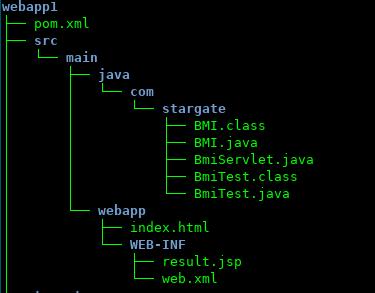
\includegraphics[scale=0.7]{/java/filetree}
\caption{\emph{"webapp1"} Projesinin Dosya Yapısı}
\label{fig:filetree}
\end{figure}
Projeyi derlemek ve hemen kullanıma koymak için maven aracını kullanmak bize büyük esneklik ve kolaylık sağlar. Altta olup bitenden çok kopmadan projenin kontrolü tamamen sizde olur. Özellikle ilk başta bir IDE kullanarak yapılan projeler genellikle ayrıntıya hakim olamama sorununa yol açabilir. 
Diğer bir yol ise javac ile derlemeleri yapıp manuel olarak classları yerlerine koymaktır ancak küçük projelerde bu yapılabilir olsa da biraz büyük projeler için ayrı bir iş yükü getireceğinden tavsiye edilmemektedir.

\subsection{Maven` a Kısa Bir Giriş}%
\label{sub:mavengiris}
C++ için \emph{make} neyse java için textbf{emph{Maven}} odur. Maven aslında  
sadece bir yapılandırma aracı (build tool) değil eklentili yapısı ile tüm projeyi
ve deployment` ı ayarlamaya ve şekillendirmeye yarayan bir araçtır.

Projenin derlenmesi için kaynak (src) klasörünün yanında \emph{pom.xml} adındaki
proje konfigurasyon dosyasının oluşturulması gerekir (Bkz. Şekil \ref{fig:filetree} ve Liste \ref{list:webpom}). Maven pom.xml dosyasında belirttiğimiz bağımlılıkları ve kütüphaneleri de otomatik olarak kurar.


\lstinputlisting[label={list:webpom},caption={Maven Yapılandırma Dosyası: pom.xml},language={XML},breaklines]{/home/cagatay/gitrepo/Ipa-ITBook/konular/java/projects/webProjects/webapp1/pom.xml}
Projeyi derlemek için pom dosyasının olduğu proje klasörü içerisinde \emph{mvn:compile} yazılır.
Projeyi server` a yüklemek için "\emph{mvn tomcat7:deploy}" veya daha önce yüklemiş ama güncellemek istiyorsak "\emph{mvn tomcat7:redploy}" yazmamız yeterlidir. Local serverımız da (http:localhost:8080/webapp1-1.0) altında projemizi inceleyebiliriz. Pom.xml içerisinde projenin yükleneceği adresi ve diğer ayarları yapabiliriz.

\subsection{Vücut Kütle Endeksi Programı, Örnek Projenin Ayakları}
Projemiz  MVC altyapısına uygun olarak biri karşılama diğeri sonuç sayfası olmak üzere iki adet seyir (view) sayfası, istekleri (request) alan işleyen ve yönlendiren bir adet servlet ve Vücut Kütle Endeksi (BMI) hesabını yapan bir adet Java (POJO) sınıfından oluşmaktadır. 

Şekil \ref{fig:servletAkis} de görüldüğü üzere arada bir de Web Container (Tomcat veya Jetty gibi bir server) bir katman daha ve bir mapping dosyası (web.xml) bulunmaktadır. 

Önce index sayfasından (Liste \ref{list:bmi_index}) servlet` e bir istek gelmekte, container tarafından bu istek çözümlenip BMI servlete iletilmektedir.
\begin{figure}[h]
\centering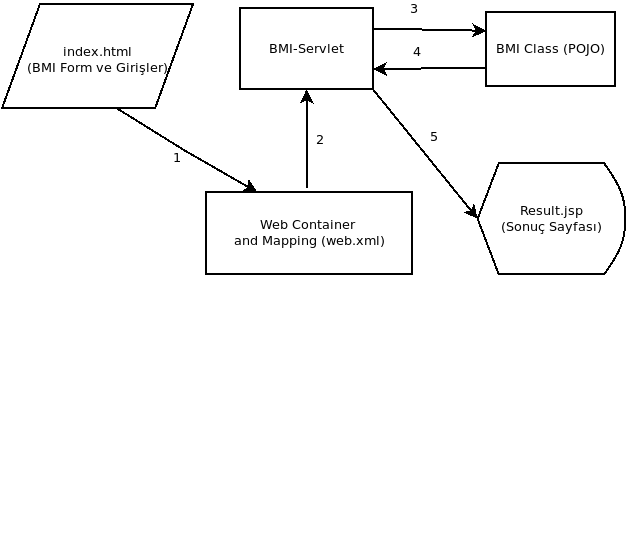
\includegraphics[scale=0.5]{/java/servlet}
\caption{Proje (webapp1) Akış Diagramı}
\label{fig:servletAkis}
\end{figure}
\lstinputlisting[label={list:bmi_index},caption={Index Sayfa Kodu},language={HTML},breaklines]{/home/cagatay/gitrepo/Ipa-ITBook/konular/java/projects/webProjects/webapp1/src/main/webapp/index.html}

